\section{\acl{ADCS}}
\label{pruneADCS}
The gravity-gradient stabilisation and passive magnetic options are eliminated because they provide insufficient accuracy and do not allow pointing to a any target other than the mass or magnetic centre of the Earth. The spin stabilisation option is pruned because the satellite needs to be able to make measurements continuously. Double gimbal \acp{CMG} are also not a viable option, because they are too complex and heavy compared to the other systems.
For the attitude determination the initial measurements and magnetometers options are eliminated because of their low accuracy over time.
The pruned design option tree can be found in figure \ref{fig:pruneADCS} on page \pageref{fig:pruneADCS}.

\begin{figure}
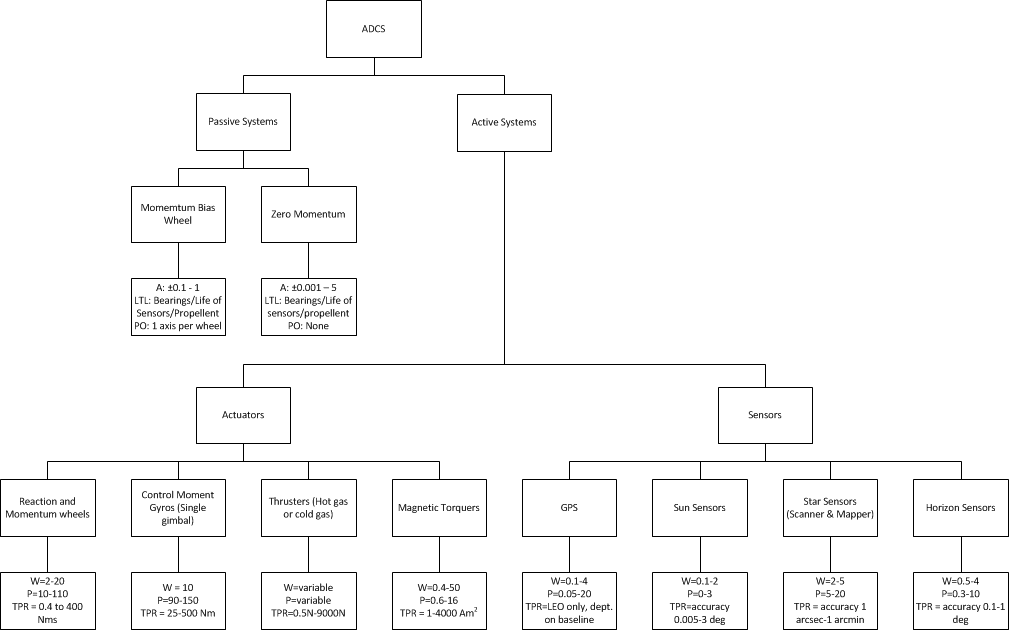
\includegraphics[width=0.8\textwidth, angle=90]{chapters/img/prunedADCStree.png}
\label{fig:pruneADCS}
\caption{Pruned design option tree for the \ac{ADCS}}
\end{figure}